\documentclass[notes,slidesec,a4]{seminar}

\usepackage[utf8]{inputenc}
\usepackage[spanish]{babel} % espanol


\usepackage{t-gsyc-6}
\usepackage{fancybox}
\usepackage{graphics}
\usepackage{moreverb}
\usepackage{alltt}
\usepackage{html}
\usepackage{color}
\usepackage[usenames,dvipsnames,svgnames,table]{xcolor}
\usepackage{amsmath}
\usepackage[normalsize]{subfigure}
\usepackage{url}
\usepackage{hyperref}
\usepackage{listings}
\usepackage{multirow}
\usepackage{hyperref}

\makeatletter
\define@key{PDF}{Movie}{\pdf@addtoks{#1}{Movie}}
\define@key{PDF}{Activation}{\pdf@addtoks{#1}{Activation}}
\newcommand{\moviewithpreview}[3]{% args: width, preview, movie
\pdfmark[{\includegraphics[width=#1]{#2}}]{%
pdfmark=/ANN,Subtype=/Movie,Movie=<< /F (#3) >>,%
Activation=<< /ShowControls true /Mode /Repeat >>}}
\newcommand{\movie}[3]{% args:width, height, movie
\pdfmark[{\hbox to #1 {\vbox to #2 { }}}]{%
pdfmark=/ANN,Subtype=/Movie,Movie=<< /F (#3) /Poster true >>,%
Activation=<< /ShowControls true /Mode /Repeat >>}}
\makeatother

\title{Aplicación web: Classcity}
\author{Mario Fernandez Guerrero}

\cop{Mario Fernández Guerrero}
\address{m.fernandezgue@alumnos.urjc.es}

\begin{document}
\maketitle


%%--------------------------------------------------------------
%%------- Transparencias de Indice
%%--------------------------------------------------------------

\begin{hslide}
\slsect{Índice}
\begin{itemize}
\item Introducción
\item Objetivos
\item Infraestructura de la aplicación
\item Implementación y desarrollo de la aplicación
\item Despliegue en la nube
\item Conclusiones
\end{itemize}
\end{hslide}

%%--------------------------------------------------------------
%%------- Transparencias de introducción
%%--------------------------------------------------------------
\begin{hslide}
\slsect{Introducción}
\begin{itemize}
\item Aplicación de gestión de clases particulares.
\item Aplicaciones que me han servido de inspiración.
\item Arquitectura de una aplicación web
\end{itemize}
\end{hslide}

%%--------------------------------------------------------------
%%------- Transparencias de Objetivos
%%--------------------------------------------------------------
\begin{hslide}
\slsect{Objetivos}
\textbf{Objetivo general: } Desarrollo y despliegue de una aplicación web que permita el contacto entre alumnos y profesores.

\textbf{Subobjetivos: }
\begin{enumerate}
\item Desarrollo del lado cliente de la aplicación.
\item Desarrollo del lado servidor de la aplicación.
\item Implementación de la base de datos.
\item Despliegue en la red.
\end{enumerate}
\end{hslide}

%%--------------------------------------------------------------
%%------- Transparencias Infraestructura
%%--------------------------------------------------------------

\begin{hslide}
\slsect{Infraestructura}
\begin{figure}
\centering
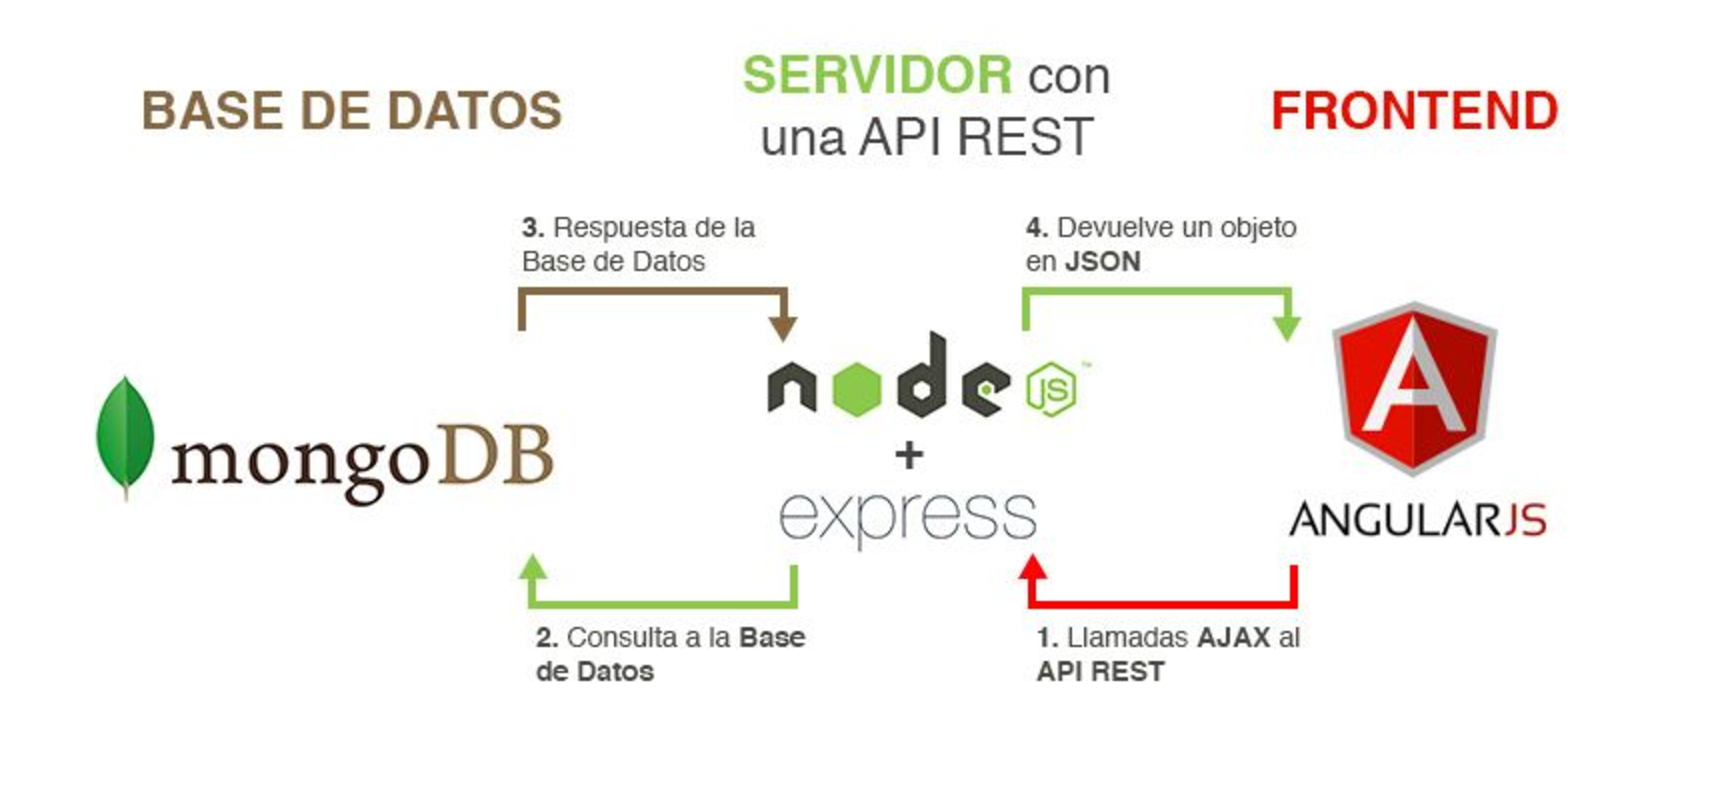
\includegraphics[width=12cm]{img/scheme.png}
\end{figure}
\end{hslide}


%%--------------------------------------------------------------
%%------- Transparencias Infraestructura
%%--------------------------------------------------------------

\begin{hslide}
\slsect{Cliente}
\textbf {Angular} framework para aplicaciones web desarrollado en TypeScript, de código abierto, mantenido por Google, que se utiliza para crear y mantener aplicaciones web de una sola página.
\begin{figure}
\centering
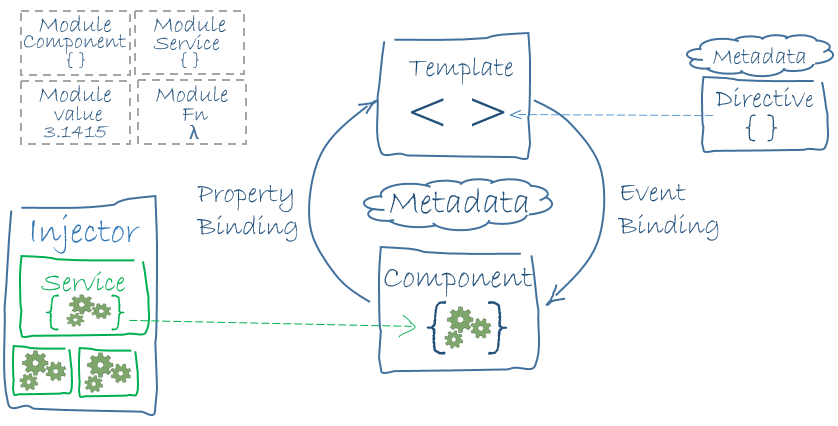
\includegraphics[width=9cm]{img/angular2Architecture.png}
\end{figure}
\end{hslide}

%%--------------------------------------------------------------
%%------- Transparencias Infraestructura
%%--------------------------------------------------------------

\begin{hslide}
\slsect{Angular}
Podemos identificar los 8 bloques principales de una aplicación web con Angular:
\begin{enumerate}
\item \textbf {Módulos}
\item \textbf {Componentes}
\item \textbf {Plantilla}
\item \textbf {Metadatos}
\item \textbf {Data Binding}
\item \textbf {Directiva}
\item \textbf {Servicio}
\item \textbf {Inyección de dependencias}
\end{enumerate}
\end{hslide}


%%--------------------------------------------------------------
%%------- Transparencias Infraestructura
%%--------------------------------------------------------------

\begin{hslide}
\slsect{Servidor}
\textbf {Node: }entorno en tiempo de ejecución multiplataforma, basado en el lenguaje de programación ECMAScript, asíncrono, con I/O de datos en una arquitectura orientada a eventos

\textbf {Express: }entorno de Node, esta diseñado para construir aplicaciones web y APIs.
\begin{enumerate}
\item \textbf {Start Server}
\item \textbf {Rutas}
\item \textbf {Controladores}
\item \textbf {Gestión del chat}
\end{enumerate}
\end{hslide}

%%--------------------------------------------------------------
%%------- Transparencias Infraestructura
%%--------------------------------------------------------------

\begin{hslide}
\slsect{Base de datos}
\textbf{MongoDB} sistema de base de datos NoSQL orientado a documentos BSON.
\begin{enumerate}
\item \textbf {Modelos}
\item \textbf {Moongoose}
\end{enumerate}
\end{hslide}

%%--------------------------------------------------------------
%%------- Transparencias Aplicación
%%--------------------------------------------------------------

\begin{hslide}
\slsect{Funcionalidades destacables en la aplicación}
\begin{enumerate}
\item Login del alumno y del profesor con credenciales cifradas.
\item Registro del alumno y del profesor con credenciales cifradas.
\item Buscar al profesor por distancia, curso y asignatura.
\item Ir al perfil del profesor.
\item Actualizar imagen de perfil del profesor.
\item Enviar solicitud de contacto a un profesor.
\item Chat.
\end{enumerate}
\end{hslide}

%%--------------------------------------------------------------
%%------- Transparencias Aplicación
%%--------------------------------------------------------------

\begin{hslide}
\slsect{Login del alumno y del profesor con credenciales cifradas.}
\begin{enumerate}
\item Petición AJAX con método POST.
\item Servidor procesa el body de la petición.
\begin{itemize}
\item Si el usuario esta registrado retorna un 201 con token y con fecha de expiración 5 minutos.
\item Si el usuario no esta registrado retorna un 401 'A user with that username already exists'.
\end{itemize}
\item El cliente procesa la respuesta del servidor, guardando en cache el token durante 5 minutos.
\end{enumerate}
\end{hslide}

%%--------------------------------------------------------------
%%------- Transparencias Aplicación
%%--------------------------------------------------------------

\begin{hslide}
\slsect{Registro del alumno y del profesor con credenciales cifradas.}
\begin{enumerate}
\item Petición AJAX con método POST.
\item Servidor procesa el body de la petición.
\begin{itemize}
\item Si el usuario consigue registrarse retorna un 201 con token cuya fecha de expiración es de 5 minutos.
\item Si el usuario ya existe retorna un 400 con el siguiente mensaje: 'A user with that username already exists'.
\item Si el usuario no introduce algún campo obligatorio el servidor responde con un 400.
\end{itemize}
\item El cliente procesa la respuesta del servidor, guardando en cache el token.
\end{enumerate}
\end{hslide}



%%--------------------------------------------------------------
%%------- Transparencias Aplicación
%%--------------------------------------------------------------

\begin{hslide}
\slsect{Buscar al profesor por distancia, curso y asignatura.}
\begin{enumerate}
\item Usuario completa parametros de busqueda y le da click a buscar.
\item Petición AJAX con método POST.
\item Servidor procesa el body y busca en la base de datos aquellos profesores que cumplan las características que se solicitan en el body.
\item El cliente procesa la respuesta del servidor y los pinta en el mapa.
\end{enumerate}
\end{hslide}

%%--------------------------------------------------------------
%%------- Transparencias Aplicación
%%--------------------------------------------------------------

\begin{hslide}
\slsect{Ir al perfil del profesor.}
\begin{enumerate}
\item Petición AJAX con método GET;
\item Servidor busca en la base de datos el profesor con su id.
\item El cliente procesa la respuesta del servidor y pinta los datos del profesor en la ficha técnica.
\end{enumerate}
\end{hslide}

%%--------------------------------------------------------------
%%------- Transparencias Aplicación
%%--------------------------------------------------------------

\begin{hslide}
\slsect{Actualizar imagen de perfil del profesor.}
\begin{enumerate}
\item Utilización de la librería 'FileUploader' en la parte cliente para poder enviar ficheros al servidor.
\item Utilización de la dependecia 'multer' para la recepción de ficheros en el servidor.
\item Guardamos en la base de datos del profesor el 'path' de la nueva imagen.
\end{enumerate}
\end{hslide}

%%--------------------------------------------------------------
%%------- Transparencias Aplicación
%%--------------------------------------------------------------

\begin{hslide}
\slsect{Enviar solicitud de contacto a un profesor.}
\begin{enumerate}
\item Cuando el alumno hace click en el botón 'Enviar notificación'
\item Se envia petición AJAX con metodo POST.
\item Actualización en la base de datos del profesor en el campo 'notification'.
\item El profesor cuando accede a su perfil verá una petición de contacto del alumno y podrá aceptar o no la solicitud.
\end{enumerate}
\end{hslide}

%%--------------------------------------------------------------
%%------- Transparencias Aplicación
%%--------------------------------------------------------------

\begin{hslide}
\slsect{Chat}
\begin{enumerate}
\item Cuando un profesor acepta una solicitud de contacto de un alumno, le da derecho a poder chatear con el.
\item El profesor tiene que estar conectado para que los alumnos puedan hablar con el.
\item Los alumnos se conectan a la sala donde el profesor esta escuchando.
\item Todos los mensajes del chat son enviados por websocket al servidor.
\item El servidor es el encargado de reeviar ese mensaje a todos los miembros que están en la sala.
\end{enumerate}
\end{hslide}

%%--------------------------------------------------------------
%%------- Transparencias Despliegue en la red
%%--------------------------------------------------------------

\begin{hslide}
\slsect{Despliegue en la nube: AWS}
\begin{enumerate}
\item Crear una instancia en AWS
\item Conectarnos por ssh a nuestra maquina virtual.
\item Correr el lado cliente en modo producción y copiar carpeta dist en la carpeta httdocs
\item Conseguir un dominio, en nuestro caso www.classcity.es
\item Correr lado servidor
\item Configurar servidor apache para redireccionar peticiones.
\end{enumerate}
\end{hslide}


%%--------------------------------------------------------------
%%------- Transparencias Conclusiones
%%--------------------------------------------------------------

\begin{hslide}
\slsect{Conclusiones}
\begin{itemize}
\item \textbf{Conclusión: } El objetivo general de desarrollar una aplicación web y desplegarla en la red se ha cubierto satisfactoriamente.
\item \textbf{Trabajos Futuros: }
\begin{enumerate}
\item WebRTC para videoconferencia.
\item Valoración de los Profesores.
\item Añadir calendarios.
\item Añadir un método de pago.
\end{enumerate}
\end{itemize}
\end{hslide}


%%--------------------------------------------------------------
%%------- Transparencias Enlaces
%%--------------------------------------------------------------
\begin{hslide}
\slsect{Enlaces}
\begin{itemize}
\item Mediawiki: \url{https://jderobot.org/Graylinx-tfg}
\item Repositorio:\\ \url{https://github.com/RoboticsURJC-students/2016-tfg-Mario-Fernandez/}
\end{itemize}
\end{hslide}

\end{document}
